\documentclass[12pt,a4paper]{article}
\usepackage[utf8]{inputenc}
\usepackage[english]{babel}
\usepackage{amsmath}
\usepackage{amsfonts}
\usepackage{amssymb}
\usepackage{graphicx}

\title{CGAD Exercise 3}
\author{Hanna Huber e0925230\\Stefan Zaufl e0925357}

\begin{document}
\maketitle
\section{Task 1}
The goal of this task was the computation of the interpolated spline of a set of points. We had a look at three methods for generating the knot vectors: equidistant, Chord and Lee. For the C1-continuity we used FMILL and Bessel to estimate the first order derivation. The different knot vector algorithms can be view in figure \ref{fig:compC1Bessel}. There is not too much difference, but this might be the case because the points are nearly equidistant to their neighbors.
The different first derivative estimations can be compared in figure \ref{fig:compC1Lee}. In our example the FMILL method looks almost like a polygonal line. The Bessel method produces much rounder transitions, but the lack of C2-continuity is clearly visible.

\begin{figure}[hbtp]
\centering
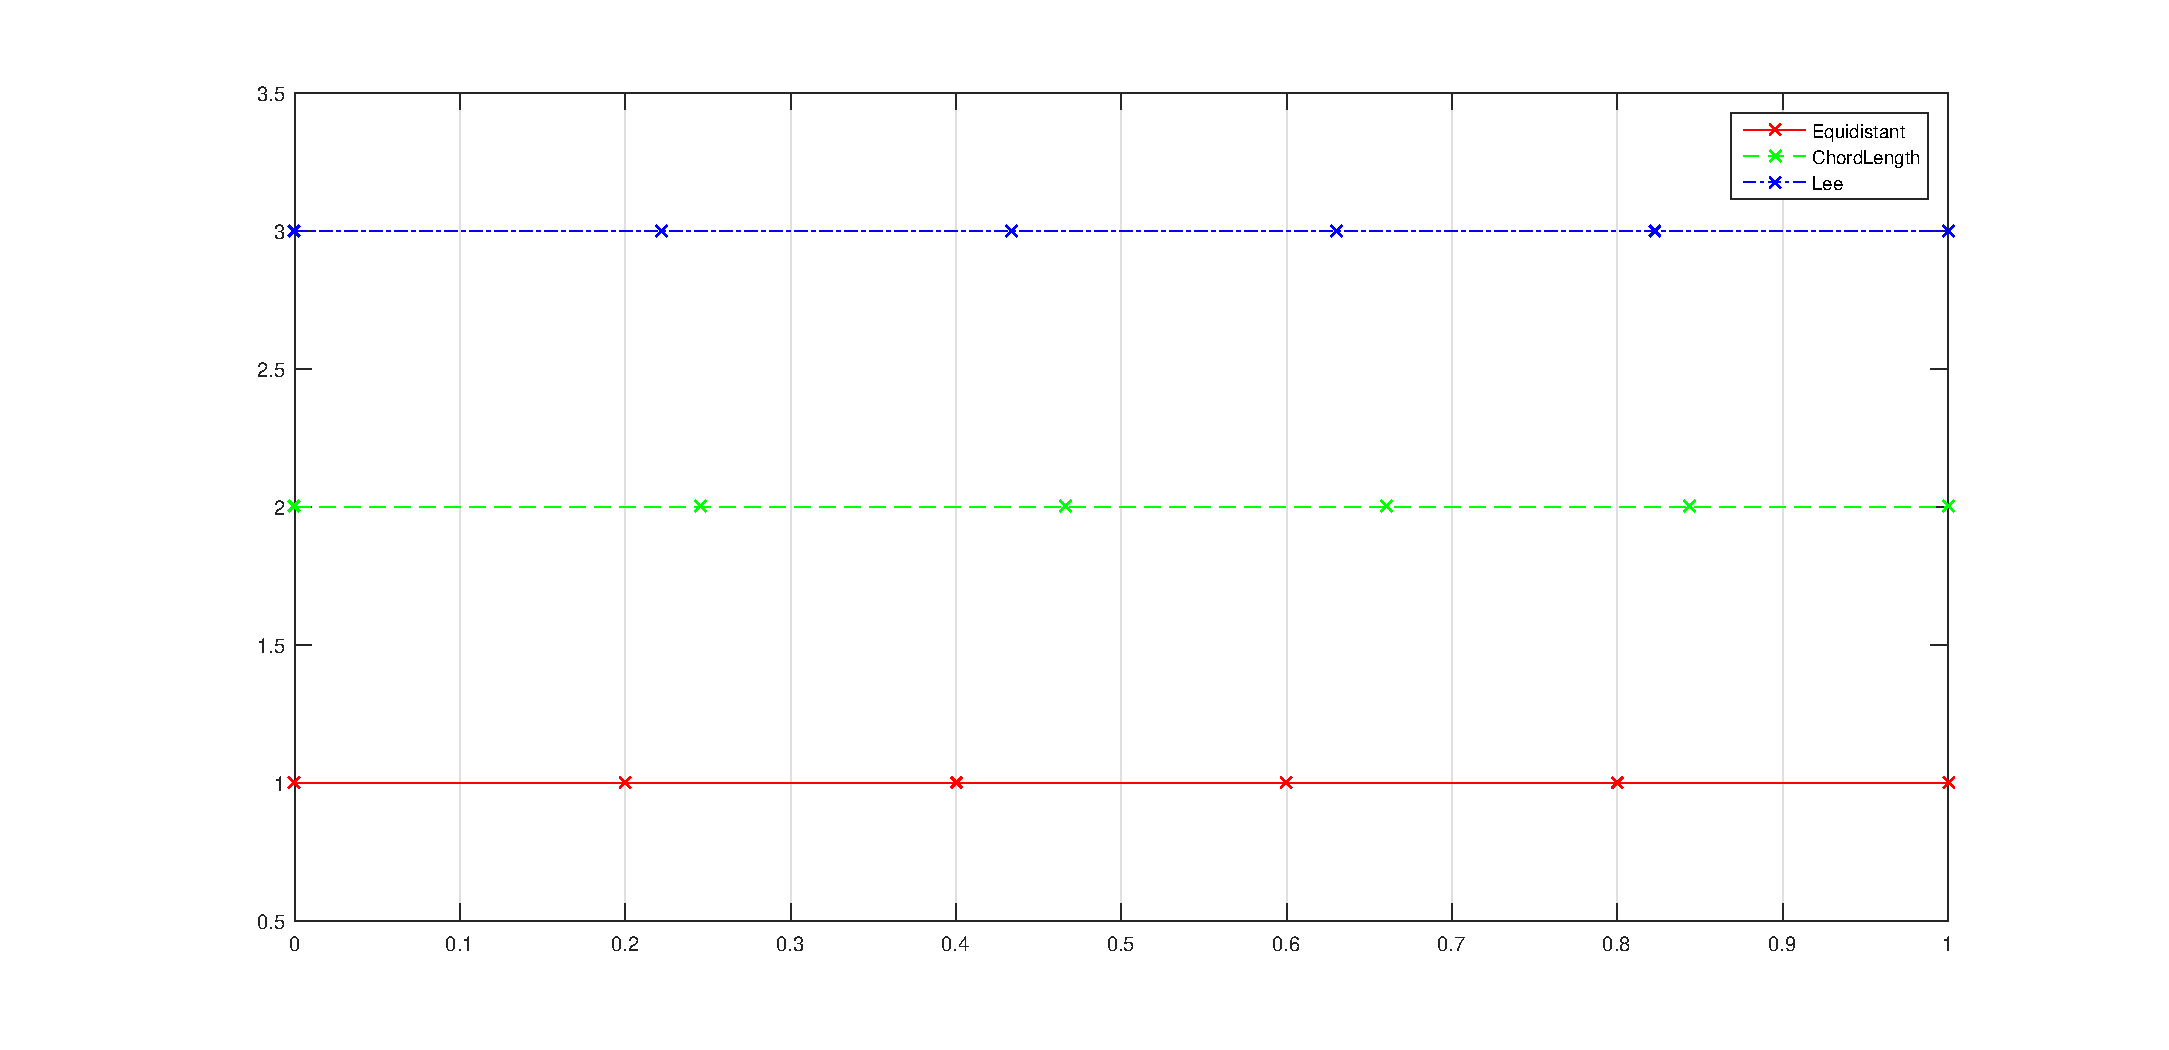
\includegraphics[width=\textwidth]{knotvectors.eps}
\caption{The different knot vectors yielded for our example curve.}
\label{fig:knotvec}
\end{figure}

\begin{figure}[hbtp]
\centering
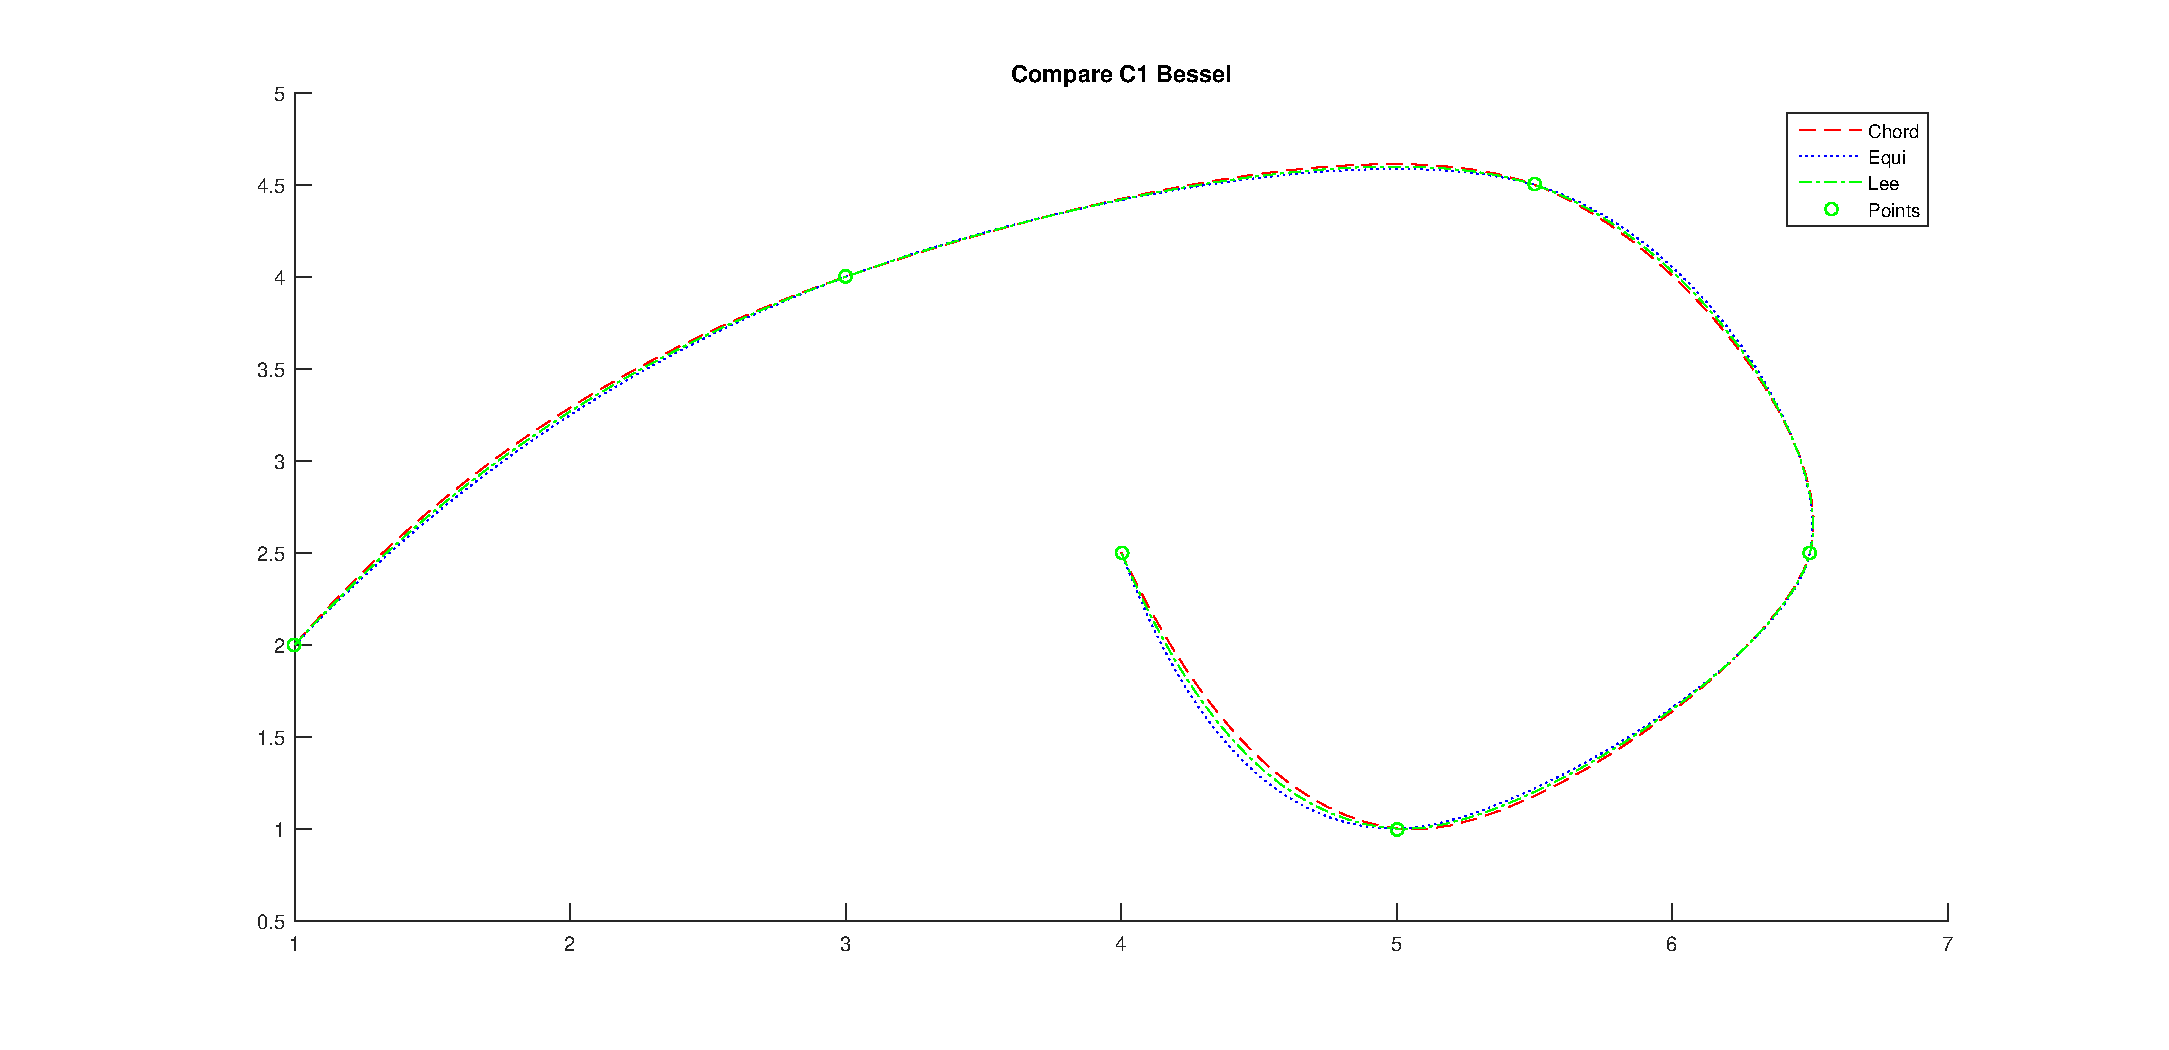
\includegraphics[width=\textwidth]{compC1Bessel.eps}
\caption{Comparison between the diffrent knot algorithms using the Bessel derivation estimation for a C1 continuity.}
\label{fig:compC1Bessel}
\end{figure}

\begin{figure}[hbtp]
\centering
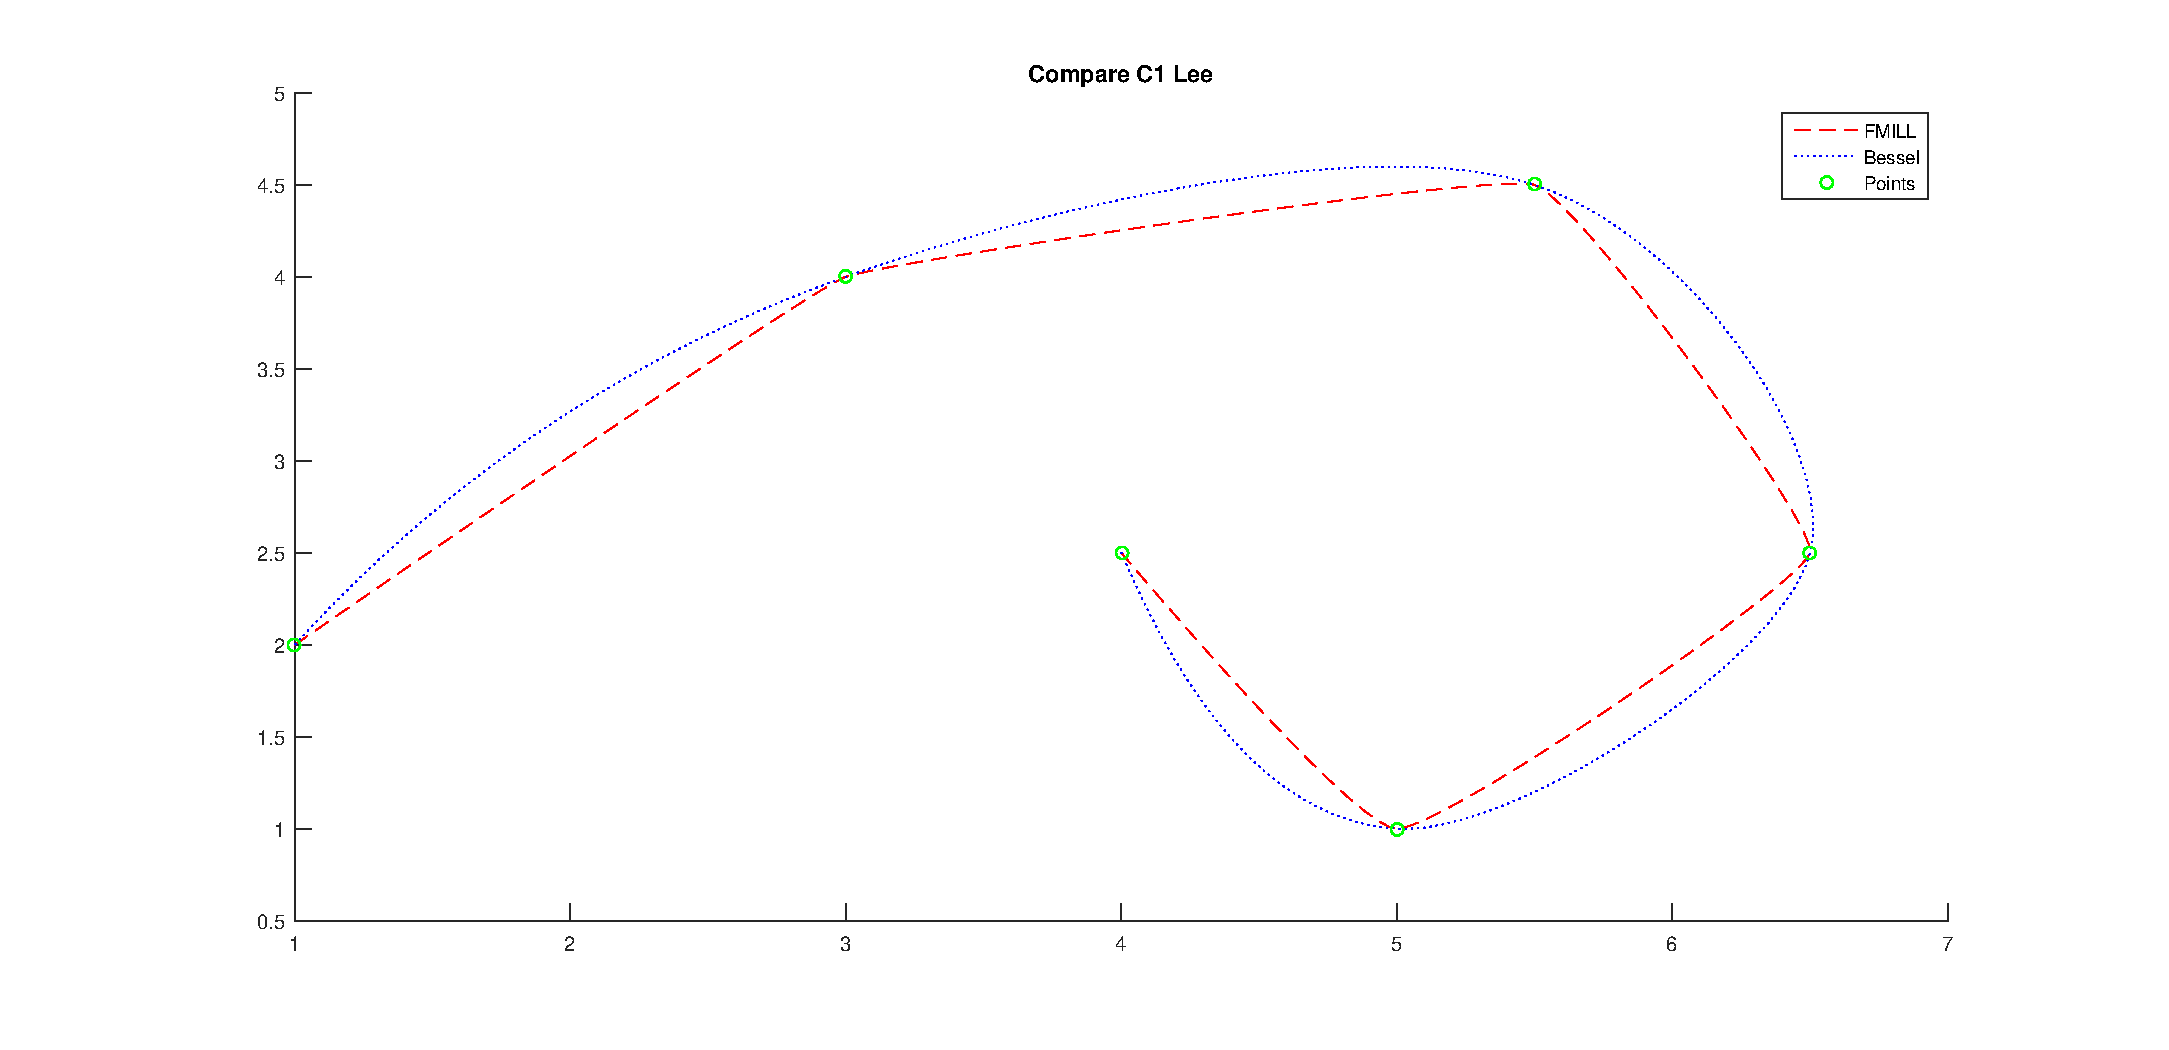
\includegraphics[width=\textwidth]{compC1Lee.eps} 
\caption{Comparison between the different derivation estimation methods for C1 continuity using the Lee knot algorithm.}
\label{fig:compC1Lee}
\end{figure}

\begin{figure}[hbtp]
\centering
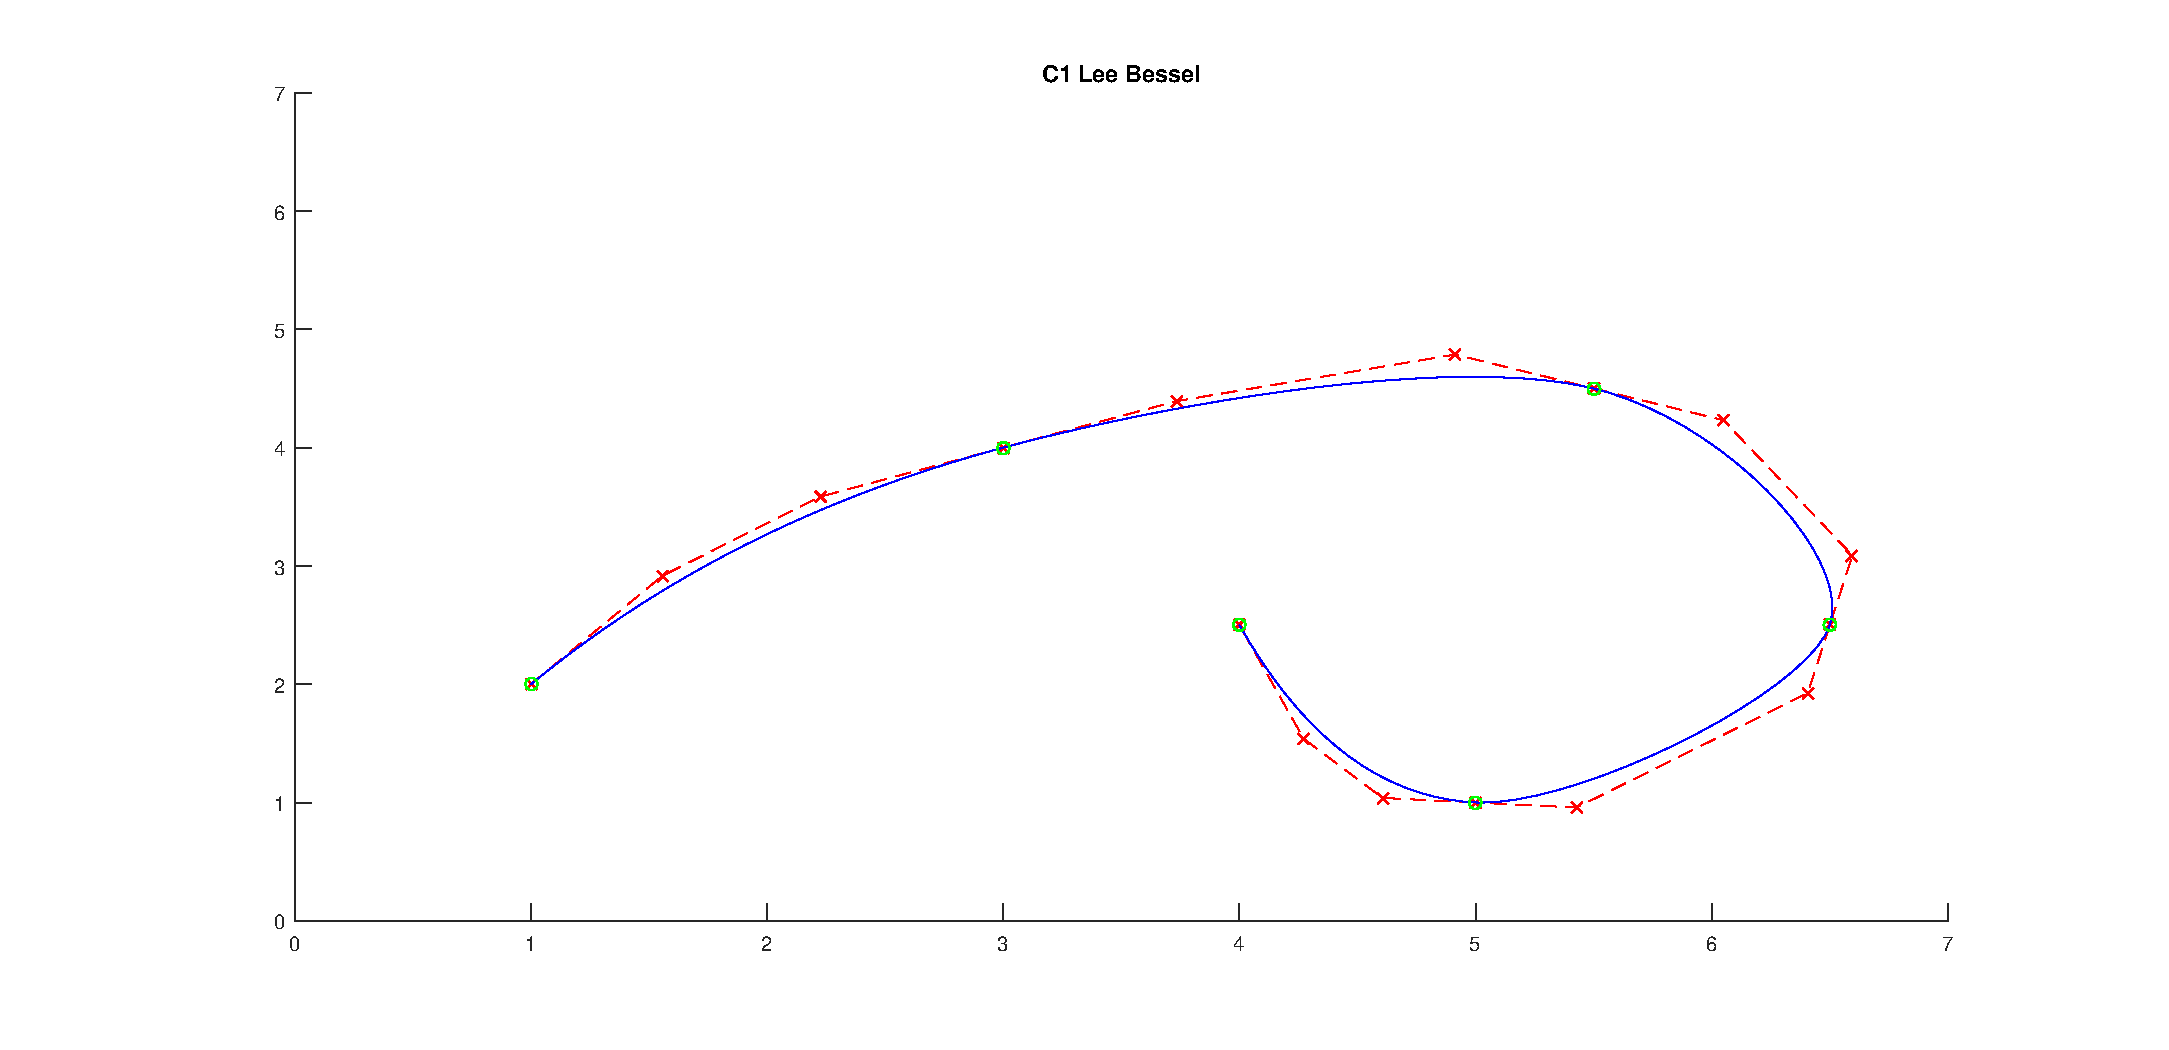
\includegraphics[width=\textwidth]{C1-LeeBessel.eps}
\caption{Showing the results of the Lee-Bessel method with the control polygons of the cubic curves.}
\label{fig:C1-LeeBessel}
\end{figure}


\end{document}